\documentclass[tikz]{standalone}
\usepackage{tikz}
\usepackage{pgfplots}
\usetikzlibrary{decorations.pathreplacing}
\begin{document}

	
	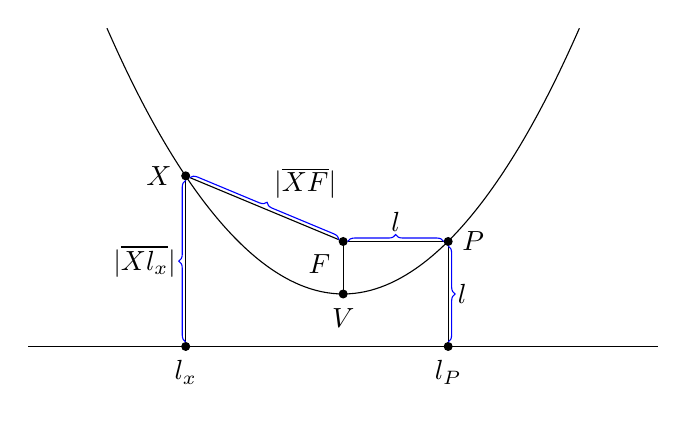
\begin{tikzpicture}[dot/.style={draw,fill,circle,inner sep=1pt}]
\draw (0,0) parabola (-3,27/8);
\draw (0,0) parabola (3,27/8);

	\node[dot,label={below left:$F$}] (F) at (0,2/3) {};
	\node[dot,label={left:$X$}] (X) at (-2,3/2) {};
	\node[dot,label={below:$V$}] (V) at (0,0) {};
	\node[dot,label={right:$P$}] (P) at (4/3,2/3) {};
	\node[dot,label={below:$l_x$}] (l) at (-2,-2/3) {};
	\node[dot,label={below:$l_P$}] (l1) at (4/3,-2/3) {};
	%\coordinate[label={above:$F$}] (F) at (0,0);
	\draw (-4,-2/3) -- (4,-2/3);
	\draw (X) -- (F);
	\draw (X) -- (l);
	\draw (F) -- (P);
	\draw (l1) -- (P);
	\draw (F) -- (V);	
	\draw[decorate,decoration=brace,draw=blue] (l) -- (X);
	\draw[decorate,decoration=brace,draw=blue] (X) -- (F);
	\draw[decorate,decoration=brace,draw=blue] (F) -- (P);
	\draw[decorate,decoration=brace,draw=blue] (P) -- (l1);
	\coordinate[label={above:$l$}] (s1) at (2/3,2/3);
	\coordinate[label={right:$l$}] (s2) at (4/3,0);
	\coordinate[label={above right:$|\overline{XF}|$}] (s3) at (-1,13/12);
	\coordinate[label={left:$|\overline{Xl_x}|$}] (s4) at (-2,5/12);
	\end{tikzpicture}
\end{document}






